\documentclass{article}
\usepackage[utf8]{inputenc}
\usepackage[russian]{babel}
\usepackage{graphicx}
\usepackage{amsmath}
\usepackage{breqn}
\usepackage{wrapfig}
\usepackage{float}
\usepackage{multirow}
\usepackage{caption}
\usepackage{subcaption}

\graphicspath{ {./data/images} }
\author{Александр Романов Б01-107}
\date{}
\title{4.5.3 Сканирующий интерферометр}

\begin{document}
\maketitle
\section{Введение}
\subsection{Цель работы}
Знакомство с устройством и работой газового лазера непрерывного действия, со спектральными характеристиками
лазерного излучения, а также с устройством и принципом действия сканирующего интерферометра Фабри—Перо.

\subsection{В работе используются}
\(He-Ne\)-лазер с блоком питания; сканирующий интерферометр Фабри—Перо; поляроид; пластинка \(\lambda / 4\); линза;
фотодиод; электронный осциллограф.

\begin{figure}[H]
  \centering
  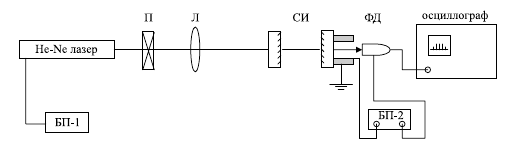
\includegraphics[width=\textwidth]{device}
  \caption{Схема экспериментальной установки}
  \label{fig:device}
\end{figure}

\begin{figure}[H]
  \centering
  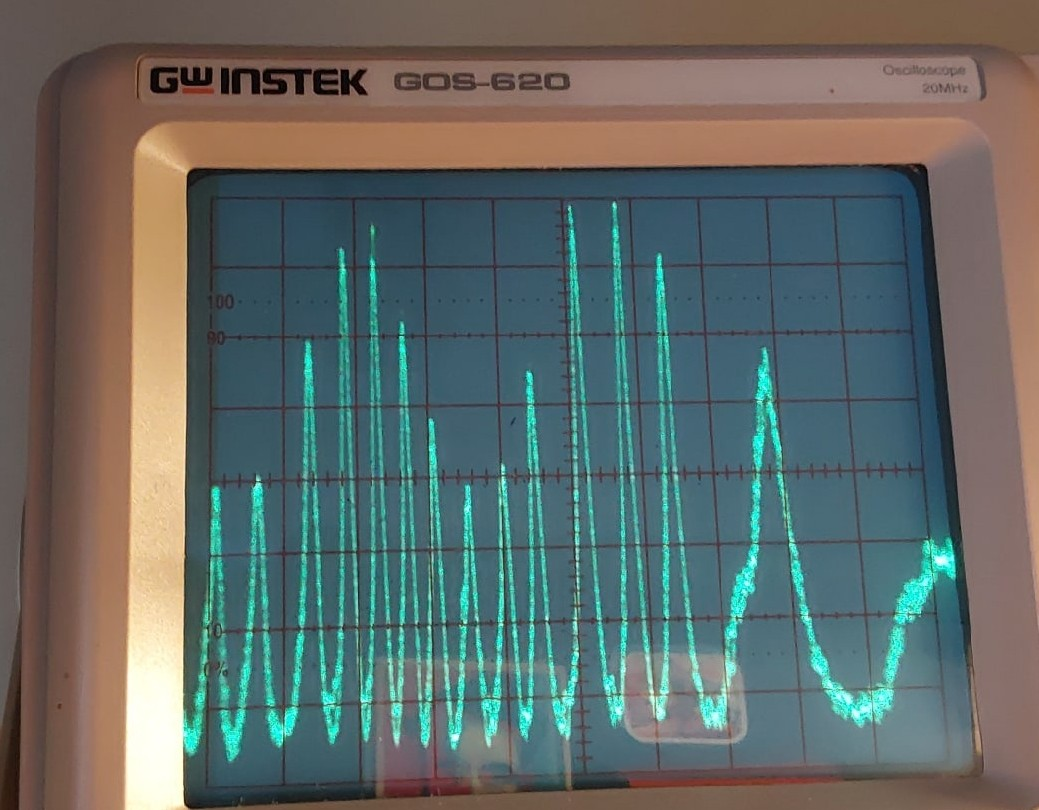
\includegraphics[width=\textwidth]{modes}
  \caption{Картина мод на осциллографе}
  \label{fig:modes}
\end{figure}

\section{Работа}
\subsection{}
Расчитаем межмодовое расстояние резонатора в единицах \(\nu\) и \(\lambda\). Длинна лазера \(L = 65\:cm\)
и \(\lambda = 632.8\cdot 10^{-9}\:m \)
\[ \Delta\nu = \nu_{m+1} - \nu_m = \frac{c}{2L} \simeq 2.3\cdot10^8\; Hz\]
\[ \Delta\lambda = \lambda{m+1} - \lambda_m = \frac{\lambda^2}{2L} = 0.3\cdot 10^{-12}\:m \]

\subsection{}
Сосчитаем на экране число промежутков между модами внутри одного доплеровского контура:
\[ N = 6 \pm 1 \]
Оценим видимую ширину спектральной линии неона:
\[ \Delta\lambda_{Ne} = \frac{m\cdot\Delta\lambda }{2} \simeq \left( 0.9 \pm 0.15  \right)\cdot 10^{-12}\:m \]  

\subsection{}
Полагая, что ширина спектральной линии обусловлена эффектом Доплера и что видимая ширина линии неона
порядка полуширины доплеровского контура 
\(\left[\Delta\lambda\left(Ne\right) \simeq \Delta\lambda_D\right]\), оценим среднюю скорость атомов 
неона вдоль оси лазера:
\[ v_x \simeq \frac{\Delta\lambda_D}{\lambda}\cdot c \simeq \left( 426 \pm 71 \right)\; m/s \]
И газокинетическую температуру (\( m = 33.5\cdot 10^{-27}\: kg\)):
\[ \frac{mv_x^2}{2} = \frac{kT}{2} \Rightarrow T = \frac{mv_x^2}{k} \simeq  \left(440 \pm 145 \right)\;K  \]

\subsection{}
Расчитаем дисперсионную область сканирующего интерферометра:
\[ \Delta\lambda_{SI} = \frac{\lambda}{m} = \frac{\lambda^2}{2l} = 
\frac{\left(632.8\cdot 10^{-9}\right)^2}{2 \cdot 0.09} \simeq 2.2\cdot 10^{-12}\;m  \]
в 2 раза больше чем \(\Delta\lambda_{Ne}\)

\subsection{}
Сравним ширину отдельной моды на полувысоте с межмодовым расстоянием. 
\[ n = 3 \pm 0.5 \]
Оценим разрешение \(\delta\lambda\) сканирующего интерферометра:
\[ \delta\lambda = \frac{\Delta\lambda}{n} \simeq \left(0.1 \pm 0.016\right)\cdot 10^{-12}\;m \]
Оценим разрешающую способность:
\[ R = \frac{\lambda}{\delta\lambda} \simeq = \left(6.328 \pm 1.012 \right)\cdot 10^6 \]

Оценим коэффициент отражения  зеркал интерферометра:
\[ R = \frac{2\pi l}{\lambda(1-r)} \Rightarrow r = 1 - \frac{2\pi l}{\lambda R} \simeq \left(0.86 \pm 0.02 \right) \]


\section{Выводы}

\end{document}